\documentclass[paper=a4, fontsize=10pt]{jlreq}

\usepackage{amsmath, amssymb}
\usepackage{enumerate}
\usepackage{tikz}
\usepackage{listings, xcolor}

\lstset{
  basicstyle = {\ttfamily},
  frame = {tbrl},
  breaklines = true,
  numbers = left,
  showspaces = false,
  showstringspaces = false,
  showtabs = false,
  keywordstyle = \color{blue},
  commentstyle = {\color[HTML]{1AB91A}},
  identifierstyle = \color{black},
  stringstyle = \color{brown},
  captionpos = t
}

\title{情報学群実験 NetworkSimulator}
\author{学籍番号 1280391 \\ 細川 夏風}
\date{\today}

\begin{document}

\maketitle
\section{実験内容}
\texttt{FTP}アプリケーションの\texttt{TCP}通信について異なる帯域幅での通信のスループット，輻輳ウィンドウ(\texttt{cwnd})，スロースタート閾値(\texttt{ssthresh})などを可視化する．
\begin{enumerate}[(a). ]
  \item 帯域幅$18$\texttt{Mbps}
  \item 帯域幅$9$\texttt{Mbps}
  \item 帯域幅$5 \sim 25$\texttt{Mbps}
  \item 帯域幅$1 \sim 5$\texttt{Mbps}
\end{enumerate}

\section{実験方法}
\subsection{帯域幅$18$\texttt{Mbps}}
\label{18Mbps}
\texttt{out.tcp}データから，\texttt{cwnd}と\texttt{ssthresh}の$2$項目を時間単位で抜き出し，それを図示する．また，スループットに対しては\texttt{out.tcp}の\texttt{cwnd}に対してパケットサイズの積をとり，最後に\texttt{rtt}で商をとるとスループットが求められる．

\subsection{帯域幅$9$\texttt{Mbps}}
この帯域幅については節\ref{18Mbps}と同じことが言える．

\subsection{帯域幅$5 \sim 25$\texttt{Mbps}}
帯域幅$5 \sim 25$\texttt{Mbps}の範囲でスループットと帯域幅の関係を図示する．また，それぞれの帯域幅についてのスループットの遷移を見る．方法として，それぞれの\texttt{cwnd}とパケットサイズの積をその時点での\texttt{rtt}で割ることにより得られる．

\subsection{帯域幅$1 \sim 5$\texttt{Mbps}}
それぞれについて，節\ref{18Mbps}と同様の方法をとり計測する．

\section{実験結果}
\subsection{帯域幅18Mbps}
$18$\texttt{Mbps}におけるウィンドウサイズの推移および\texttt{Throughput}の計測結果を図\ref{fig:result_18mbps}に示す。

\begin{figure}[htbp]
  \begin{minipage}[b]{0.48\textwidth}
    \centering
    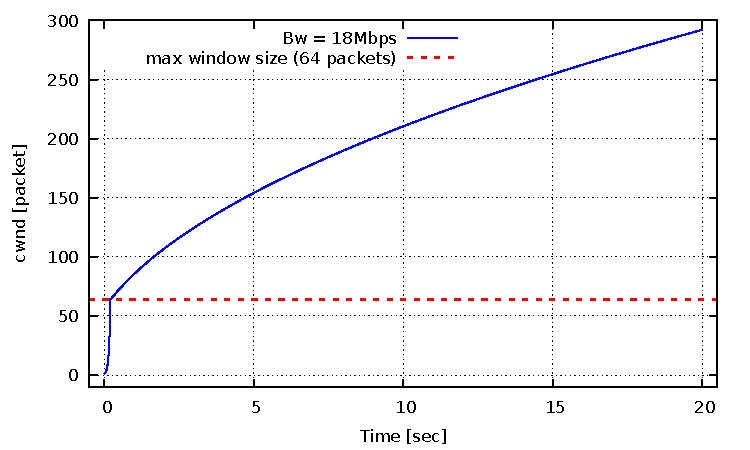
\includegraphics[width=\textwidth]{kadai2-1-a/kadai2-1-a-1.pdf}
    \caption{\texttt{cwnd} vs \texttt{Time} ($18$\texttt{M})}
  \end{minipage}
  \hfill
  \begin{minipage}[b]{0.48\textwidth}
    \centering
    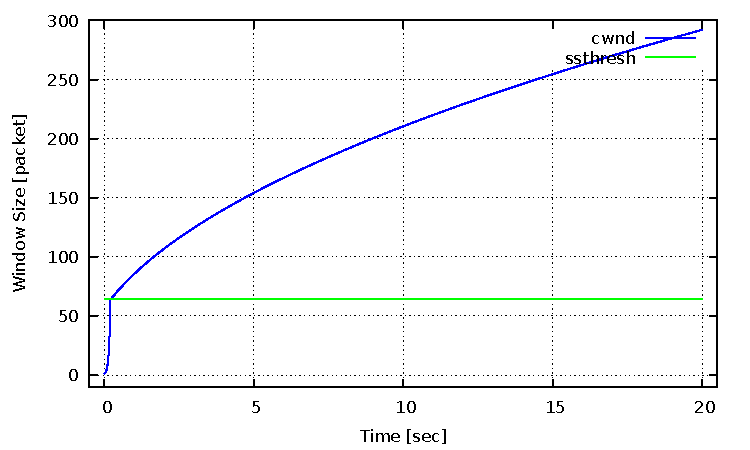
\includegraphics[width=\textwidth]{kadai2-1-a/kadai2-1-a-2.pdf}
    \caption{\texttt{cwnd}/\texttt{ssthresh} vs \texttt{Time} ($18$\texttt{M})}
  \end{minipage}
  \\
  \begin{minipage}[b]{0.48\textwidth}
    \centering
    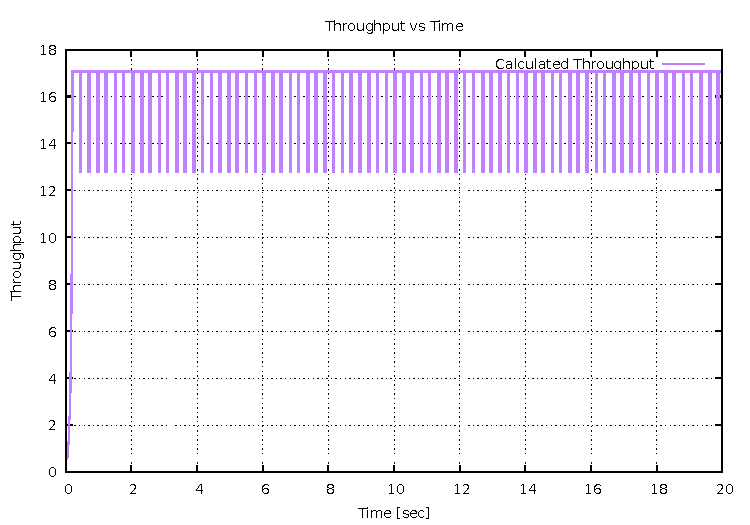
\includegraphics[width=\textwidth]{kadai2-1-a/throughput_18Mb.pdf}
    \caption{\texttt{Throughput} ($18$\texttt{M})}
  \end{minipage}
  \caption{帯域幅$18$\texttt{Mbps}における各推移}
  \label{fig:result_18mbps}
\end{figure}

\newpage

\subsection{帯域幅$9$\texttt{Mbps}}
$9$\texttt{Mbps}における各推移を図\ref{fig:result_9mbps}に示す。

\begin{figure}[htbp]
  \begin{minipage}[b]{0.48\textwidth}
    \centering
    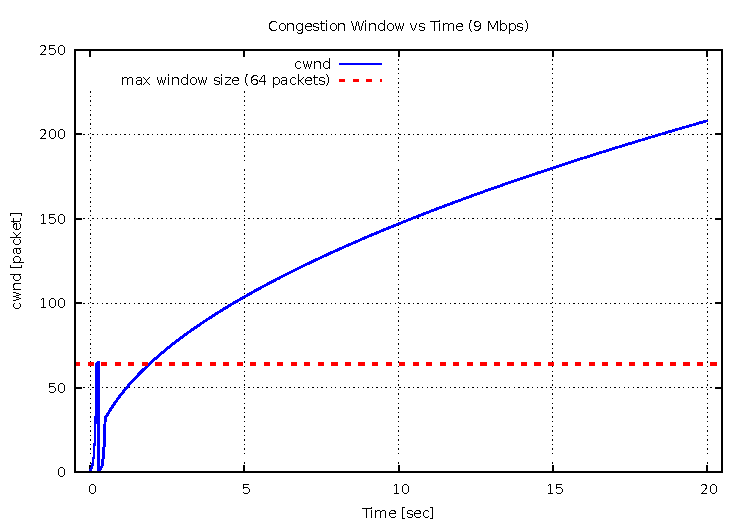
\includegraphics[width=\textwidth]{kadai2-1-b/kadai2-1-b-1.pdf}
    \caption{\texttt{cwnd} vs \texttt{Time} ($9$\texttt{M})}
  \end{minipage}
  \hfill
  \begin{minipage}[b]{0.48\textwidth}
    \centering
    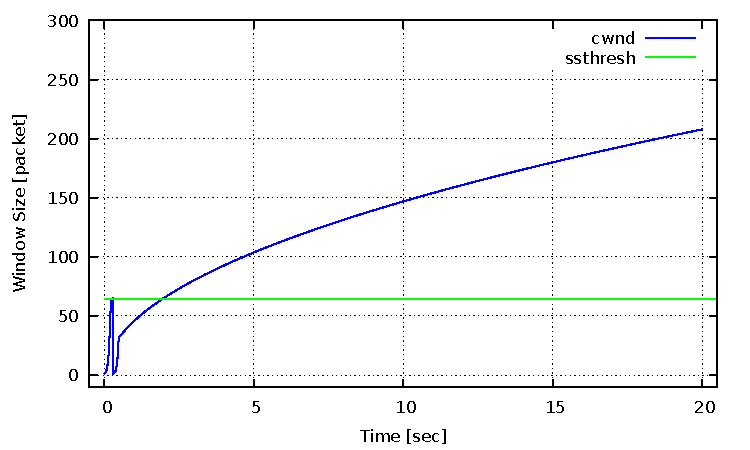
\includegraphics[width=\textwidth]{kadai2-1-b/kadai2-1-b-2.pdf}
    \caption{\texttt{cwnd}/\texttt{ssthresh} vs \texttt{Time} ($9$\texttt{M})}
  \end{minipage}
  \\
  \begin{minipage}[b]{0.48\textwidth}
    \centering
    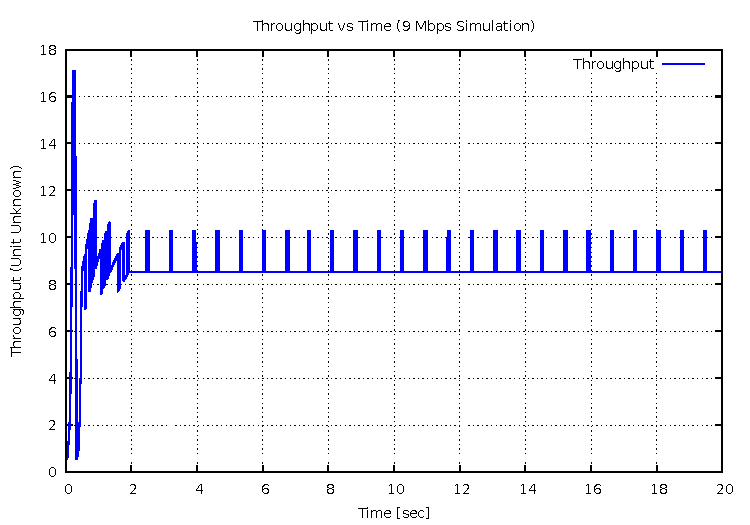
\includegraphics[width=\textwidth]{kadai2-1-b/throughput_9Mb.pdf}
    \caption{\texttt{Throughput} ($9$\texttt{M})}
  \end{minipage}
  \caption{帯域幅$9$\texttt{Mbps}における各推移}
  \label{fig:result_9mbps}
\end{figure}

\subsection{帯域幅$5 \sim 25$\texttt{Mbps}}
帯域幅を変化させた場合の\texttt{Throughput}特性を図\ref{fig:tp_c_main}に、各帯域における時系列\texttt{Throughput}を図\ref{fig:tp_c_grid}に示す。

\begin{figure}[htbp]
  \centering
  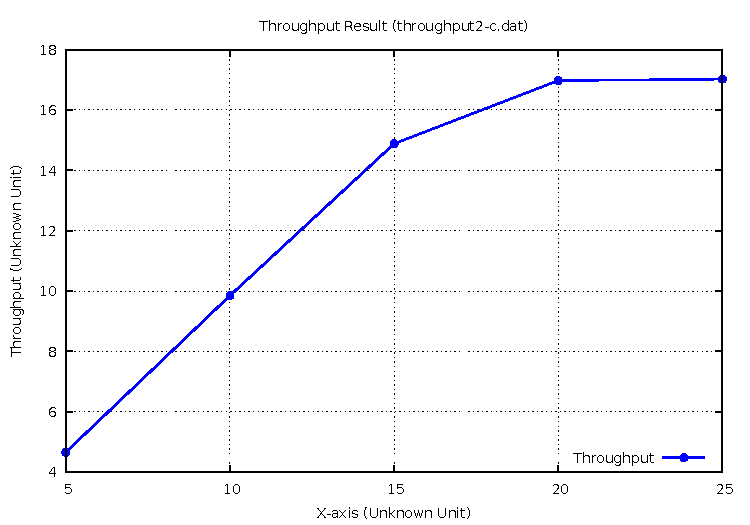
\includegraphics[width=8cm]{kadai2-1-c/throughput2-c.pdf}
  \caption{\texttt{Throughput} vs 帯域幅 ($5$-$25$\texttt{Mbps})}
  \label{fig:tp_c_main}
\end{figure}

\begin{figure}[htbp]
  \centering
  \begin{minipage}{0.32\textwidth}
    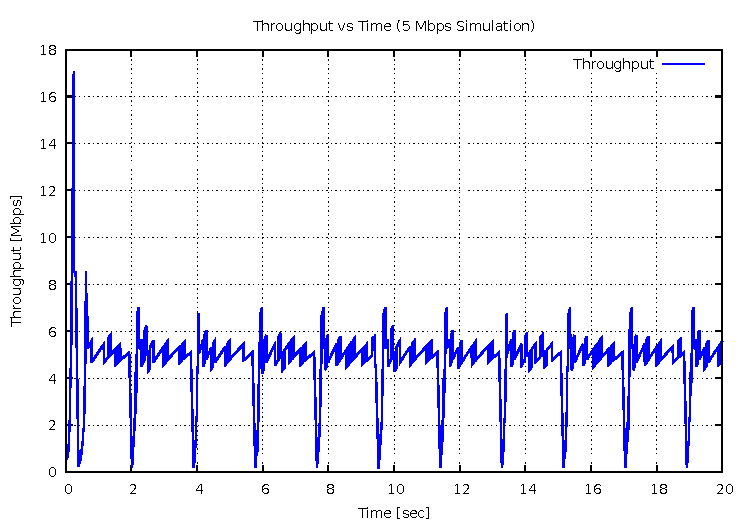
\includegraphics[width=\textwidth]{kadai2-1-c/throughput_5Mb.pdf}
    \caption*{$5$\texttt{Mbps}}
  \end{minipage}
  \begin{minipage}{0.32\textwidth}
    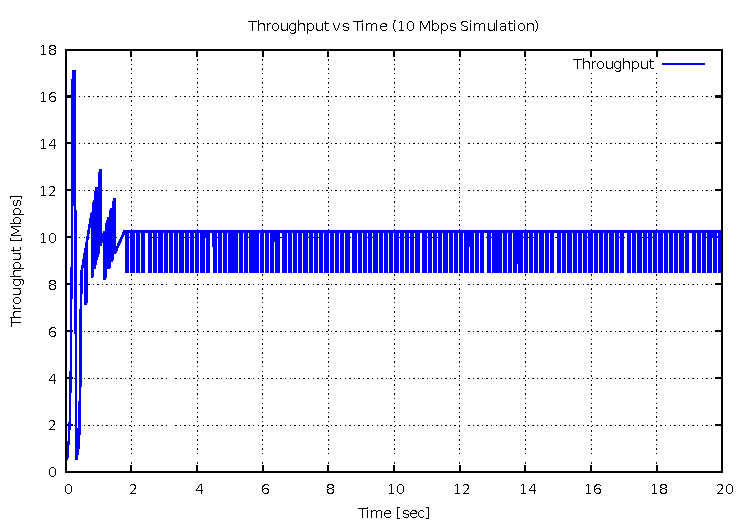
\includegraphics[width=\textwidth]{kadai2-1-c/throughput_10Mb.pdf}
    \caption*{$10$\texttt{Mbps}}
  \end{minipage}
  \begin{minipage}{0.32\textwidth}
    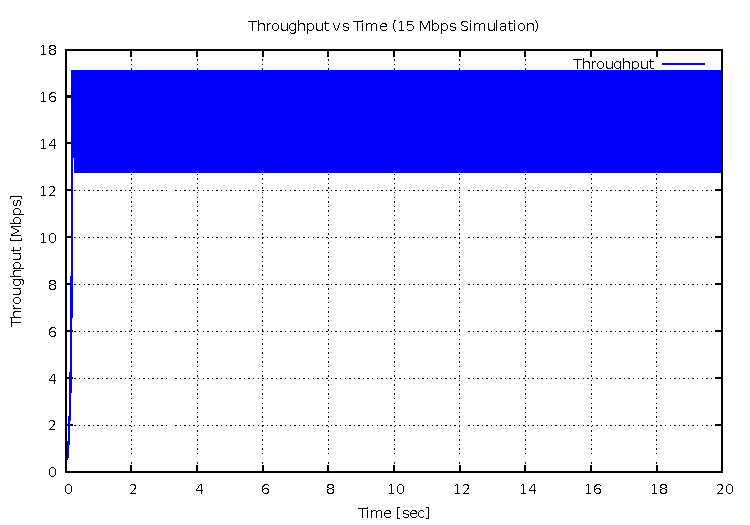
\includegraphics[width=\textwidth]{kadai2-1-c/throughput_15Mb.pdf}
    \caption*{$15$\texttt{Mbps}}
  \end{minipage}
  \\
  \begin{minipage}{0.32\textwidth}
    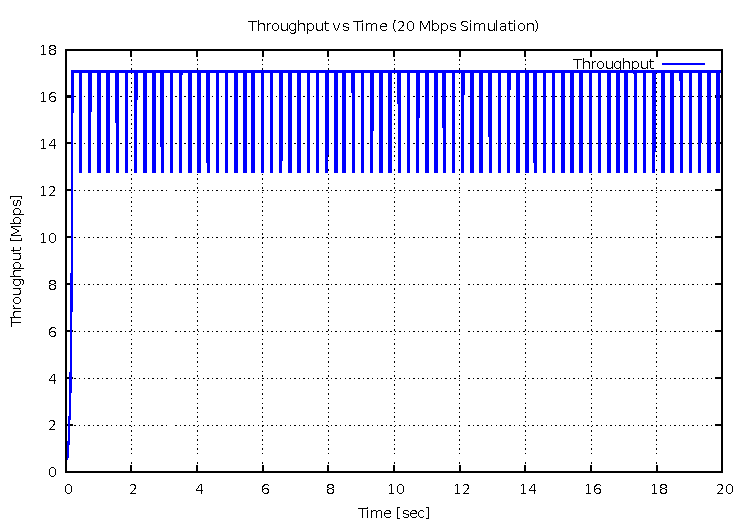
\includegraphics[width=\textwidth]{kadai2-1-c/throughput_20Mb.pdf}
    \caption*{$20$\texttt{Mbps}}
  \end{minipage}
  \begin{minipage}{0.32\textwidth}
    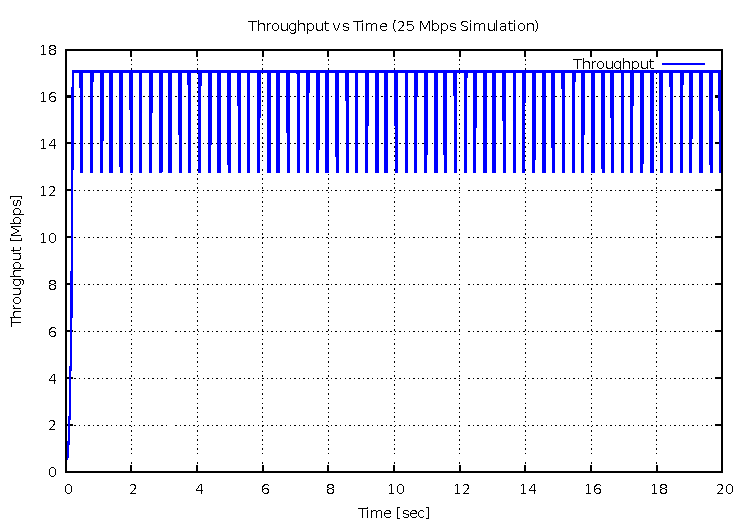
\includegraphics[width=\textwidth]{kadai2-1-c/throughput_25Mb.pdf}
    \caption*{$25$\texttt{Mbps}}
  \end{minipage}
  \caption{各帯域における\texttt{Throughput}遷移}
  \label{fig:tp_c_grid}
\end{figure}

\newpage

\subsection{帯域幅$1 \sim 5$\texttt{Mbps}}
$1 \sim 5$\texttt{Mbps}における比較結果を図\ref{fig:tp_d_main}に、それぞれの輻輳ウィンドウ推移をグリッド表示で図\ref{fig:cwnd_d_grid}および図\ref{fig:ssthresh_d_grid}に示す。

\begin{figure}[htbp]
  \centering
  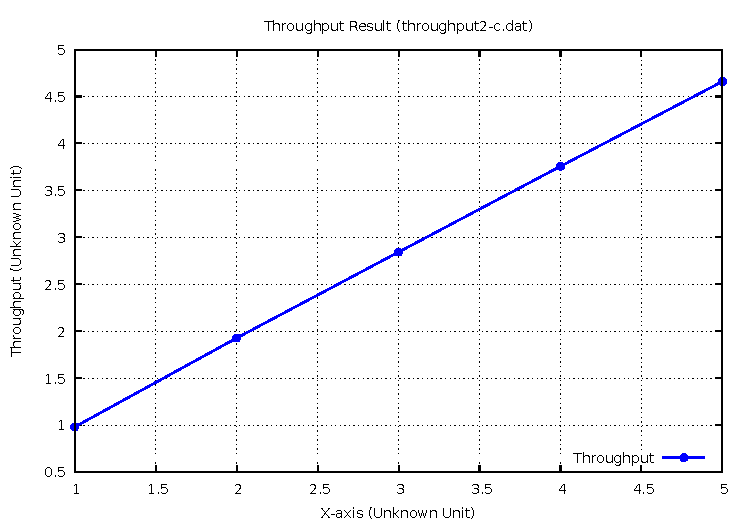
\includegraphics[width=8cm]{kadai2-1-d/throughput2-1-d.pdf}
  \caption{\texttt{Throughput} vs 帯域幅 ($1$-$5$\texttt{Mbps})}
  \label{fig:tp_d_main}
\end{figure}

\begin{figure}[htbp]
  \centering
  \begin{minipage}{0.19\textwidth}
    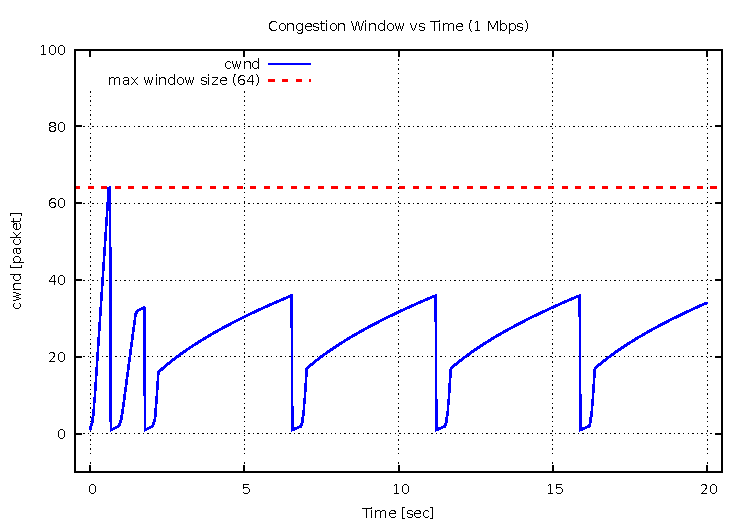
\includegraphics[width=\textwidth]{kadai2-1-d/graph1_cwnd_1Mb.pdf}
  \end{minipage}
  \begin{minipage}{0.19\textwidth}
    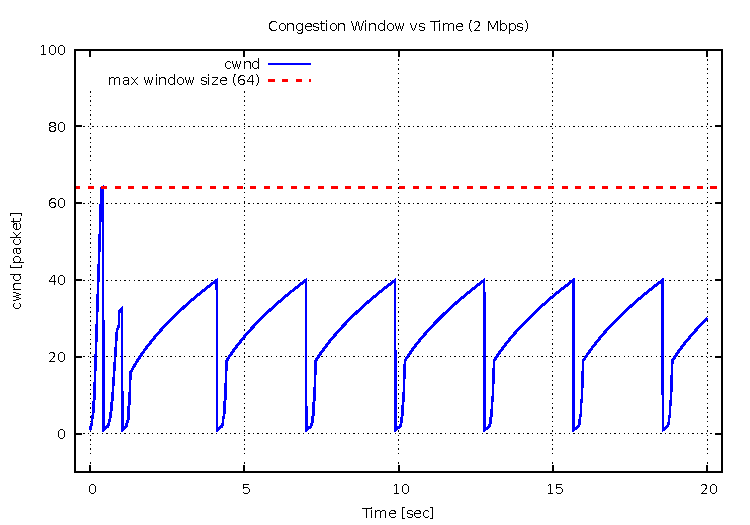
\includegraphics[width=\textwidth]{kadai2-1-d/graph1_cwnd_2Mb.pdf}
  \end{minipage}
  \begin{minipage}{0.19\textwidth}
    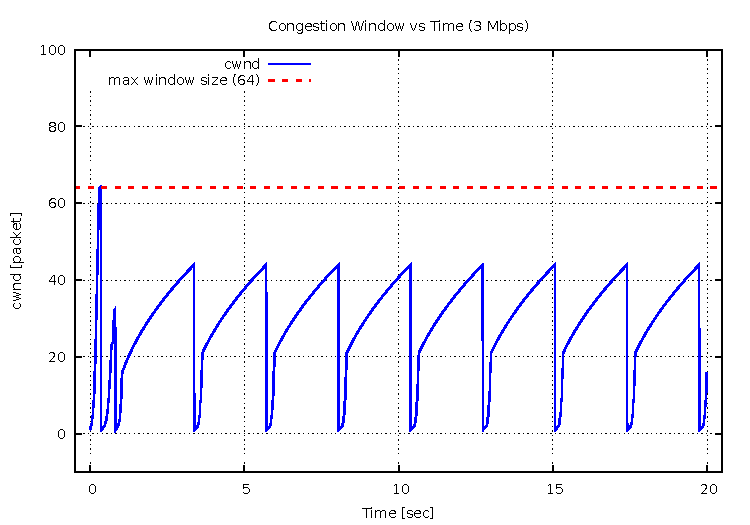
\includegraphics[width=\textwidth]{kadai2-1-d/graph1_cwnd_3Mb.pdf}
  \end{minipage}
  \begin{minipage}{0.19\textwidth}
    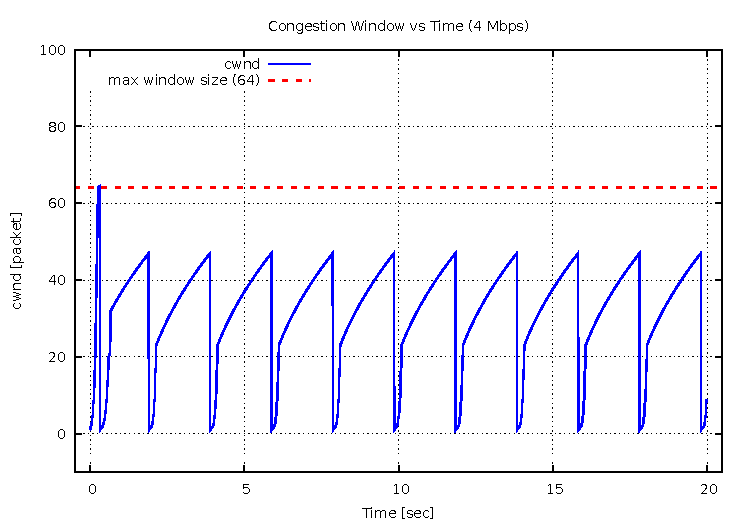
\includegraphics[width=\textwidth]{kadai2-1-d/graph1_cwnd_4Mb.pdf}
  \end{minipage}
  \begin{minipage}{0.19\textwidth}
    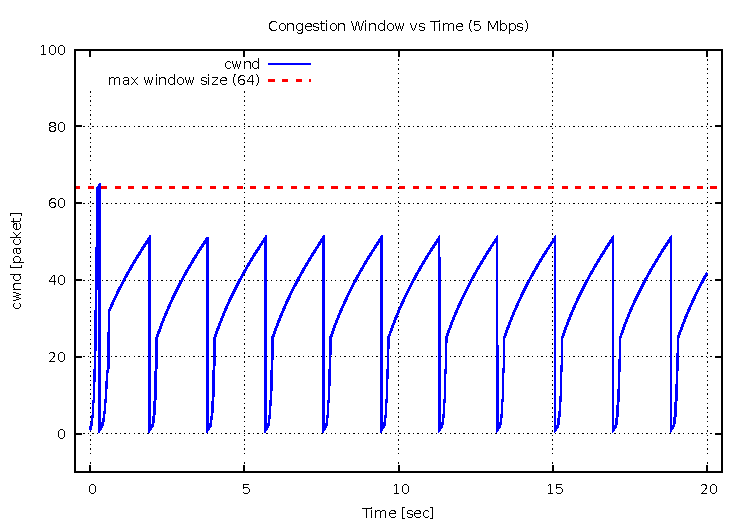
\includegraphics[width=\textwidth]{kadai2-1-d/graph1_cwnd_5Mb.pdf}
  \end{minipage}
  \caption{帯域幅$1$～$5$\texttt{Mbps}における\texttt{cwnd}の推移比較}
  \label{fig:cwnd_d_grid}
\end{figure}

\begin{figure}[htbp]
  \centering
  \begin{minipage}{0.19\textwidth}
    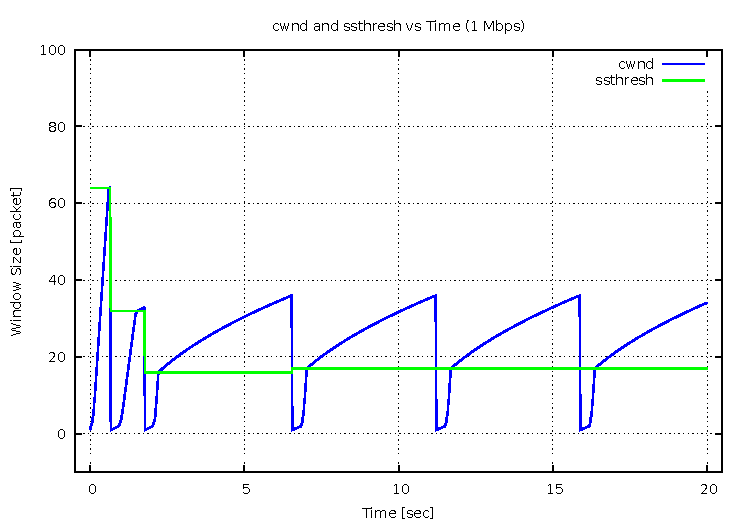
\includegraphics[width=\textwidth]{kadai2-1-d/graph2_cwnd_ssthresh_1Mb.pdf}
  \end{minipage}
  \begin{minipage}{0.19\textwidth}
    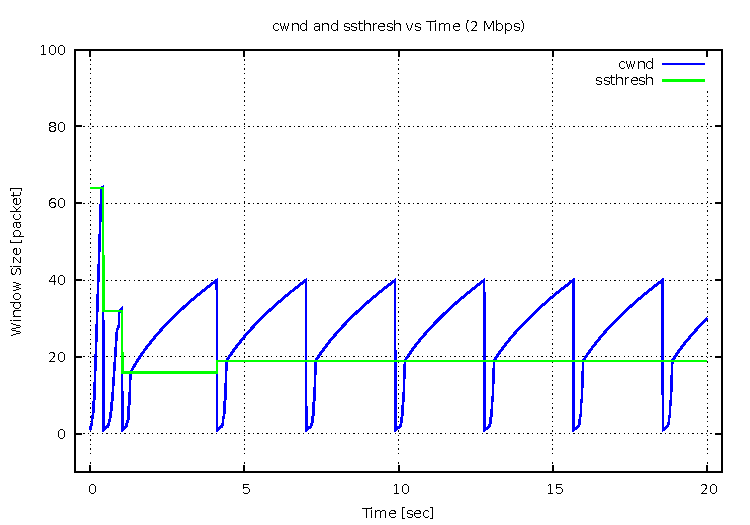
\includegraphics[width=\textwidth]{kadai2-1-d/graph2_cwnd_ssthresh_2Mb.pdf}
  \end{minipage}
  \begin{minipage}{0.19\textwidth}
    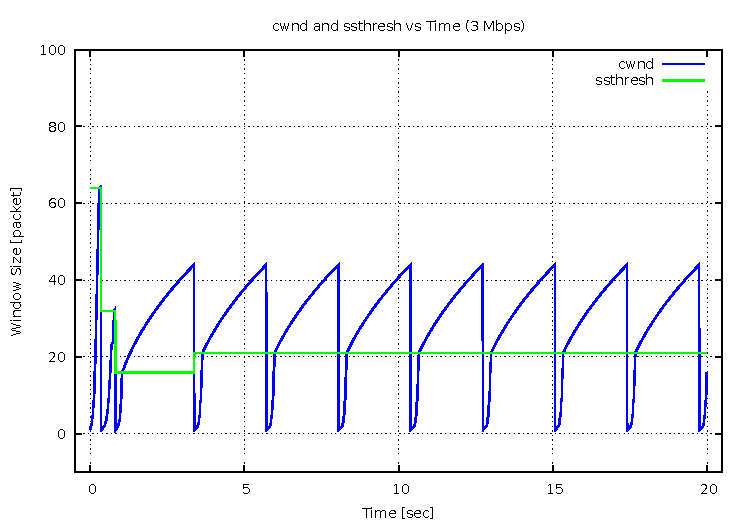
\includegraphics[width=\textwidth]{kadai2-1-d/graph2_cwnd_ssthresh_3Mb.pdf}
  \end{minipage}
  \begin{minipage}{0.19\textwidth}
    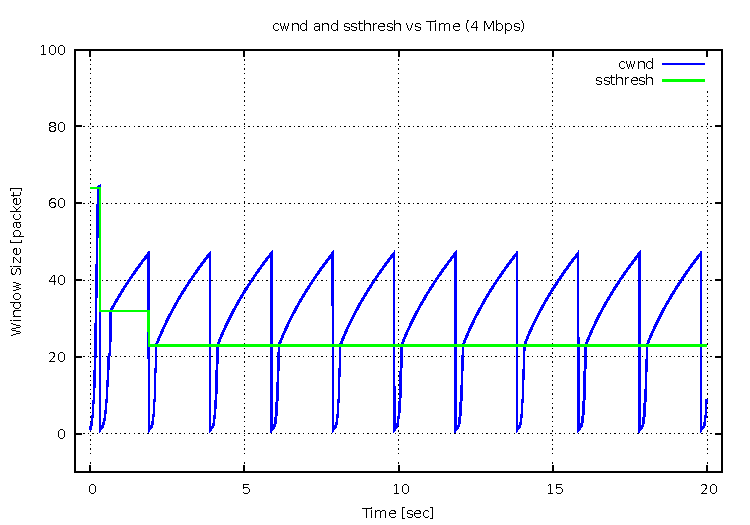
\includegraphics[width=\textwidth]{kadai2-1-d/graph2_cwnd_ssthresh_4Mb.pdf}
  \end{minipage}
  \begin{minipage}{0.19\textwidth}
    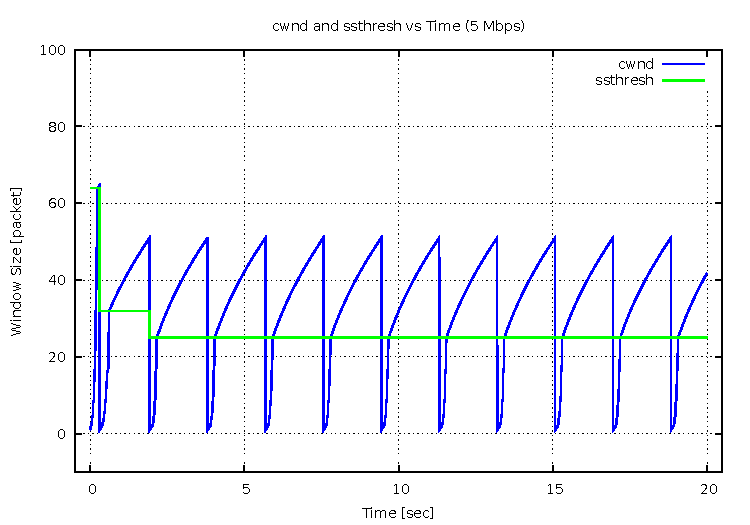
\includegraphics[width=\textwidth]{kadai2-1-d/graph2_cwnd_ssthresh_5Mb.pdf}
  \end{minipage}
  \caption{帯域幅$1$～$5$\texttt{Mbps}における\texttt{cwnd}/\texttt{ssthresh}の推移比較}
  \label{fig:ssthresh_d_grid}
\end{figure}

\newpage

\section{考察}
以上のでーたを整理し，各項目ごとに考察を述べる．
\subsection{帯域幅$18$\texttt{Mbps}}
帯域幅$18$\texttt{Mbps}は通信路としては十分であり，パケットがドロップするようなケースは見受けられなかった．また，パケット送信の最大値を超えて\texttt{cwnd}は増加しているように見える．しかし，実際には送信されているのは最大のウィンドウサイズ分である．また，\texttt{ssthresh}を超えた部分から\texttt{cwnd}の増加幅が変化してることがわかる．スループットのデータについても$12 \sim 14$の値を振動している．このことからこの帯域幅では主にこの幅で通信が行われていることがわかる．
\subsection{帯域幅$9$\texttt{Mbps}}
このデータでは$1$度タイムアウトが起こっていることがわかる．\texttt{cwnd}が$1$度$1$まで下降しているからである．また，このデータではスループットは$7 \sim 10$の値をとっており，これは帯域幅との関係からありえないことである．しかし，計算結果としてこの結果となった理由は\texttt{out.tcp}内のデータの\texttt{rtt}のデータが少数第$3$以下が$0$になっているつまり，誤差を大きすぎるためであると考えられる．
\subsection{帯域幅$5 \sim 25$\texttt{Mbps}}
スループットは$20 \sim 25$にかけて上昇していないか，上昇量が微々たるものであることがわかる．これは帯域幅が送信データより多くなったためであると考えられる．蛇口とそれにつながってるホースの関係に例えられる．中に水が流れる場合のようにホースの太さが十分である時それ以上ホースを太くしても効果が上がることは無い．そのような関係からどの通信においても上昇幅は送信データの大きさに近づくにつれて小さくなる．また，時間あたりのスループットの関係からパケットの損失率が小さいほどきれいな図になることがわかる．また，帯域幅が大きくなるにつれて変動が少なくなっていることがわかる．これは先程と同様のことから説明できる．

\subsection{帯域幅$1 \sim 5$\texttt{Mbps}}
この帯域幅は通信には十分ではなくスループットが常に上昇していることがわかる．また，時間あたりのスループットについてはタイムアウトの回数が帯域幅が大きくなるごとに多くなっている事がわかる．これは輻輳制御が適切に行われているため，通信を適切に制御できているからであると考えられる．証拠に全体のスループットは小さい．また，\texttt{ssthresh}については変化してることがわかる．図ではこの閾値についても徐々に上昇していることがうかがえる．そのため，前述の通り制御が正確に行われてると考えられる．

\begin{thebibliography}{99}
  \bibitem{}
\end{thebibliography}

\end{document}
